This chapter will lay down the general notations and definitions required for the later parts of the thesis.
In~\cref{sec:pre:general}, we will define several cryptographic primitives which are necessary for our constructions.
\Cref{sec:pre:bitcoin} will describe definitions around Bitcoin, mainly its transaction structure.
After that, in~\cref{sec:pre:privacy}, we will discuss the notion of Privacy-enhancing cryptocurrencies and range proofs in~\cref{sec:pre:rangeproof}.
Both are essential to understand the Mimblewimble protocol addressed in~\cref{sec:pre:mimblewimble}.
Finally, we explain the concept of Scriptless Scripts and Adaptor signatures in~\cref{sec:pre:scriptless-scripts}, which are relevant building blocks for the constructions found in this thesis.

\section{General Notation and Definitions}\label{sec:pre:general}
\paragraph{Notation}
We first define the general notation used in the following chapters to formalize procedures and protocols.
Let $\cnstGroup$ denote a cyclic group of prime order $\varPrime$ and $\cnstIntegersPrime{\varPrime}$ the ring of integers modulo $\varPrime$ with identity element $\cnstIdentityElement$.
$\cnstIntegersPrimeWithoutZero{\varPrime}$ is $\cnstIntegersPrime{\varPrime} \opExcluding \funList{0}$.
$\varG \opSeperate \varH$ are adjacent generators in $\cnstGroup$, where adjacent means the discrete logarithm of $\varH$ regarding $\varG$ is not known.
Exponentiation stands for repeated application of the group operation.
We define the group operation between two curve points as $\funGen{\varScA} \opAddPoint \funGen{\funGen{\varScB}} \opEq \funGen{\varScA \opAddScalar \varScB}$.

\begin{definition}[Hard Relation]\label{def:pre:hard-relation}
    Given a language $\varLanguage \opAssign \funList{\varBigA \opForWhich \exists\varSmallA \text{ s.t. } (\varBigA, \varSmallA) \opIn \cnstRelation}$ then the relation $\cnstRelation$ is
    considered hard if the following three properties hold:~\cite{aumayr2020bitcoinchannels}
    \begin{enumerate}
        \item $(\varWit, \varStatement) \opFunResult \procGenR{\varSecParam}$ is a $\cnstPolyTime$ sampling algorithm which outputs a statement/witness of the form $(\varWit, \varStatement) \opIn \cnstRelation$.
        \item Relation $\cnstRelation$ is poly-time decidable.
        \item For all $\cnstPolyTime$ adversaries $\cnstAdversary$ the probability of finding $\varWit$ given $\varStatement$ is negligible.
    \end{enumerate}
\end{definition}

\begin{definition}[Discrete Logarithm]\label{def:pre:discretelog}
    We define the discrete logarithm in a group $\cnstGroup$ of a number $\varN$ as the number $\varM$ such that for the groups generator $\varG$ the following holds:
    \[ \funGen{\varM} \opEqNoQ \varN \]
    The discrete logarithm is a hard relation as defined in~\cref{def:pre:hard-relation}.
\end{definition}

\begin{definition}[Signature Scheme]\label{def:pre:signature-scheme}
    A Signature Scheme $\varSigScheme$ is a tuple of algorithms $(\procSetupId \opSeperate \procSignId \opSeperate \procVerfId)$ defined as follows:~\cite{goldwasser1988digital}
    \[ \varSigScheme = (\procSetupId \opSeperate \procSignId \opSeperate \procVerfId) \]

    \begin{itemize}
        \item $\varKeyPair \opFunResult \procSetup{\varSecParam}$: The keygen function creates a keypair $\varKeyPair$, the public key $\varPubKey$ can be distributed to the verifier(s) and the secret key $\varSecKey$ has to be kept private. \\
        \item $\varSignature \opFunResult \procSign{\varMsg}{\varSecKey}$: The signing algoritm creates a signature under the message $\varMsg$, which can be verified with the respective public key $\varPubKey$.
        As an input it takes a message $\varMsg$ and the secret key $\varSecKey$ of the signer.
        \item $\cnstTrueorFalse \opFunResult \procVerf{\varMsg}{\varSignature}{\varPubKey}$: The verification function allows a verifier knowing the signature $\varSignature$, message $\varMsg$ and the provers public key $\varPubKey$ to verify a signatures
        validity. \\
    \end{itemize}

    A valid Signature Scheme has to fulfill two security properties:
    \begin{itemize}
        \item Correctness: For all messages $\varMsg$ and valid keypairs $\varKeyPair$ the following must hold with overwhelming probability: $\procVerf{\varPubKey}{\procSign{\varSecKey}{\varMsg}}{\varMsg} \opEqNoQ 1$
        \item Unforgeability (\cnstEUFCMA): Informally the existential unforgeability under chosen message attacks holds if attacker $\cnstAdversary$ cannot forge a valid signature for a chosen message.
        More formally, for a polytime adversary $\cnstAdversary$, message $\varMsg$, and public key $\varPubKey$ the following must hold:
        \[ \varSignature \opFunResult \cnstAdversary(\varMsg, \varPubKey), \varProbability(\procVerf{\varMsg}{\varSignature}{\varPubKey} \opEqNoQ 1) \opSmEq \funNegl{\cdot} \]
    \end{itemize}
\end{definition}

\begin{definition}[Cryptographic Hash Function]\label{def:pre:hash-function}
    A cryptographic hash function $\cnstHash$ is defined as $\funHash{\varInput} \rightarrow \cnstBinary{\varN}$ for some fixed number $\varN$ and some input $\varInput$ ~\cite{al2011cryptographic}.
    A secure hashing function has to fulfill the following security properties:
    \begin{itemize}
        \item Collision-Resistance (CR): Collision-Resistance means that it is computationally infeasible to find two inputs $\varInput_1$ and $\varInput_2$ such that
        $\funHash{\varInput_1} \opAssign \funHash{\varInput_2}$ with $\varInput_1 \opNotEq \varInput_2$.
        \item Pre-image Resistance (Pre): In a hash function $\cnstHash$ that fulfills Pre-image Resistance it is infeasible to recover the original input $\varInput$ from its hash output $\funHash{\varInput}$.
        If this security property is achieved, the hash function is said to be non-invertible.
        \item 2nd Pre-image Resistance (Sec):  This property is similar to Collision-Resistance and is sometimes referred to as \textit{Weak Collision-Resistance}.
        Given such a hash function $\cnstHash$ and an input $\varInput$, it should be infeasible to find a different input $\funStar{\varInput}$ such that $\varInput \opNotEq \funStar{\varInput}$
        and $\funHash{\varInput} \opEqNoQ \funHash{\funStar{\varInput}}$.
    \end{itemize}
    The relation between the input $\varInput$ and the output $\funHash{\varInput}$ is a hard relation as defined in~\cref{def:pre:hard-relation}.
\end{definition}

\begin{definition}[Commitment Scheme]\label{def:pre:commitment}
    A cryptographic Commitment Scheme $\varCommitScheme$ is defined by a pair of functions $(\procSetupComId, \procCommitId)$~\cite{bunz2018bulletproofs}.
    \begin{itemize}
        \item $\varCommitParams \opFunResult \procSetupCom{\varSecParam}$: The setup procedure is a DPT function, it takes as input a security parameter $\varSecParam$ and outputs public parameters $\varPublicParam$.
        Depending on $\varPublicParam$ we define a input space $\varInputSpace_{\varPublicParam}$, a randomness space $\varRandSpace_{\varPublicParam}$ and a commitment space $\varCommitSpace_{\varPublicParam}$.
        \item $\varCommitment \opFunResult \procCommit{\varInput}{\varNonce}$ The commit routine is DPT function that takes an arbitrary input $\varInput \opIn \varInputSpace_{\varPublicParam}$, a random value $\varNonce \opIn \varRandSpace_{\varPublicParam}$ and
        generates an output $\varCommitment \opIn \varCommitSpace_{\varPublicParam}$.
    \end{itemize}

    Secure commitments must fulfill the \emph{Binding} and \emph{Hiding} security properties:
    \begin{itemize}
        \item \textit{Binding:} If a Commitment Scheme is binding it must hold that for all $\cnstPolyTime$ adversaries $\cnstAdversary$ given a valid input $\varInput \opIn \varInputSpace_{\varPublicParam}$
        and randomness $\varNonce \opIn \varRandSpace_{\varPublicParam}$ the probabilty of finding a $\funStar{\varInput} \opNotEq \varInput$ and a $\funStar{\varNonce}$ with
        $\procCommit{\varInput}{\varNonce} \opEqNoQ \procCommit{\funStar{\varInput}}{\funStar{\varNonce}}$ is negligible.
        \item \textit{Hiding:} For a $\cnstPolyTime$ adversary $\cnstAdversary$, commitment inputs $\varInput_0, \varInput_1 \opIn \varInputSpace_{\varPublicParam}$ randomness $\varNonce \opIn
       \varRandSpace_{\varPublicParam}$ and a commitment output $\varCommitment \opAssign \procCommit{\varInput_{\varB}, \varNonce}$ the probabilty of the adversary choosing the correct $\varB$ out of $\{0,1\}$
        must not be higher then $\frac{1}{2} + \funNegl{\varProbability}$.
    \end{itemize}
\end{definition}

\begin{definition}[Additive Homomorphic Commitment]\label{def:pre:homo-com}
    A Commitment Scheme as defined in~\cref{def:pre:commitment} is said to be addtive homomorphic if the following holds~\cite{bunz2018bulletproofs}
    \[ \procCommit{\varInput_1}{\varNonce_1} \opAddPoint \procCommit{\varInput_2}{\varNonce_2} \opEqNoQ \procCommit{\varInput_1 \opAddScalar \varInput_2}{\varNonce_1 \opAddScalar \varNonce_2} \]
\end{definition}

\begin{definition}[Pedersen Commitment Scheme]\label{def:pre:pedersen}
    A \emph{Pedersen Commitment Scheme} is an instance of a Commitment Scheme as defined in~\cref{def:pre:commitment} that has the additive homomorphic property as defined in~\cref{def:pre:homo-com}.

This can be achieved as follows:
    $\varCommitSpace_{\varPublicParam} \opAssign \cnstGroup$ of order $\varPrime \opSeperate \varInputSpace_{\varPublicParam} \opSeperate \varRandSpace_{\varPublicParam} \opAssign \cnstIntegersPrime{\varPrime}$.
    the procedures $(\procSetupComId, \procCommitId)$ are then instantiated as:
    \begin{gather*}
        \varCommitParams \opFunResult \procSetupComPed{\varG}{\varH} \opAssign \varG, \varH \opFunResult (\varG, \varH)\\
        \varCommitment \opFunResult \procCommit{\varInput}{\varNonce} \opAssign \funGen{\varNonce} \funGenH{\varInput}\\
    \end{gather*}
    An instantiation of the Pedersen Commitment Scheme must pick two adjacent generators $\varG$, $\varH$ for the setup to be secure in terms of hiding and binding.
    Formally adjacent means that there exists a hard relation between $\varG$ and $\varH$ in terms of the discrete logarithm~\cref{def:pre:discretelog}.
That means no $\varX$ is known such that $\varH \opEqNoQ \funGen{x}$.
    In practice, this is often achieved by hashing $\varG$ and using the hash output as $\varH$.

\end{definition}

To prove our protocols' security, we define the notion of security in the presence of malicious adversaries, which may deviate from the protocol arbitrarily.
To construct the definition, we must first explain two terms: $\cnstIdeal$, the execution in the ideal model and $\cnstReal$, and the real model's execution.
The following definitions are based on a tutorial paper on simulation proofs by Yehuda Lindell~\cite{lindell2017simulate}.

\paragraph{Execution in the Ideal Model} We have two parties $\varParty{1}$ with input $\varX$ and $\varParty{2}$ with input $\varY$ that cooperate to compute a two-party functionality $\cnstFunction : \cnstBinary{*} \opX \cnstBinary{*} \rightarrowtail \cnstBinary{*} \opX \cnstBinary{*}$.
The adversary $\cnstAdversary$ either controls $\varParty{1}$ or $\varParty{2}$.
The ideal execution $\cnstIdeal$ relies on the assumption that we have access to a trusted third party (TTP) and proceeds in the following steps:

\begin{enumerate}
    \item \textbf{Inputs:} The input of $\varParty{1}$ is $\varX$, and the input of $\varParty{2}$ is $\varY$.
    Both parties get an additional auxiliary input $\varZ$.
    We note that we can generalize the concept to functions that require multiple inputs or even functions which do not require any input.
    In the case of multiple inputs, the inputs of $\varParty{1}$ would then b a list $\funArray{\varX_i}$ and the inputs of $\varParty{2}$ a list $\funArray{\varY_i}$.
    For simplicity, we here describe the case with one single parameter provided by each party.
    \item \textbf{Send Inputs:} The honest party (the one which is not controlled by $\cnstAdversary$) sends its input $\varX$ (resp. $\varY$) to the trusted third party.
    The malicious party can either abort the execution by sending the symbol $\cnstAbort$ to the trusted third party, send its input $\varX$ (resp. $\varY$), or send an arbitrarily chosen string $\varK$ with the same length as $\varX$ to proceed with the protocol execution.
    The decision is made by $\cnstAdversary$ and may depend on the input or auxiliary input $\varZ$.
    We denote $(\funStar{\varX}, \funStar{\varY})$ as the inputs received by the trusted third party.
    If $\varParty{1}$ is malicious then $(\funStar{x}, \funStar{y}) \opEqNoQ (\varK, \varY)$, if $\varParty{2}$ is malicious then $(\funStar{x}, \funStar{y}) \opEqNoQ (\varX, \varK)$.
    \item \textbf{Abort:} If the trusted third party has received $\cnstAbort$ from one of the parties, then it sends $\cnstAbort$ to both parties.
    \item \textbf{Answer to Adversary:} After having received both inputs the trusted third party computes $\cnstFunction(\funStar{\varX}, \funStar{\varY}) \opEqNoQ (\cnstFunction_1(\funStar{\varX}, \funStar{\varY}), \cnstFunction_2(\funStar{\varX}, \funStar{\varY}))$ and proceeds by sending $\cnstFunction_1(\funStar{\varX}, \funStar{\varY})$ (respective $\cnstFunction_2(\funStar{\varX}, \funStar{\varY})$) to the adversary.
    \item \textbf{Adversary Instructs Trusted Party:} $\cnstAdversary$ now again has the option of sending $\cnstAbort$ to the trusted third party to stop the execution.
    Otherwise, it may send $\cnstContinue$ which means the output $\cnstFunction_1(\funStar{\varX}, \funStar{\varY})$ (respective $\cnstFunction_2(\funStar{\varX}, \funStar{\varY})$) will be delivered to the honest party.
    \item \textbf{Outputs:} The honest party outputs the answer of the trusted third party. The malicious party may output an arbitrary function of its input, the auxiliary string $\varZ$, or the answer for the trusted party.
\end{enumerate}

Let $\cnstAdversary$ be a non-uniform PPT algorithm, and $\varI \opIn \{1,2\}$ be the corrupted party's index.
We then denote $\cnstIdeal_{\cnstFunction, \styleFunction{P}(\varZ), \varI}(\varX, \varZ)$ as the ideal execution of $\cnstFunction$ on inputs $(\varX, \varY)$ with auxiliary input $\varZ$ to $\cnstAdversary$ and security param $\varSecParam$ defined as the output pair of the honest party and $\cnstAdversary$ from the ideal execution.

\paragraph{Execution in the Real Model} Again let $\cnstAdversary$ be a non-uniform PPT adversary and $\varI \opIn \{1,2\}$ be the corrupted party's index.
In this model, a real two-party protocol $\varProtocol$ is executed, but the adversary $\cnstAdversary$ sens alls messages in place of the corrupted party and may follow an arbitrary polynomial-time strategy.
Then the real execution of the two-party protocol $\varProtocol$ between $\varParty{1}$ and $\varParty{2}$ on inputs $(\varX, \varY)$ and auxiliary input $\varZ$ to $\cnstAdversary$ and security parameter $\varSecParam$ is denoted by $\cnstReal_{\cnstFunction, \styleFunction{P}(\varZ), \varI}(\varX, \varZ)$ and is defined as the output pair of the honest party and the adversary $\cnstAdversary$ from the real execution of $\varProtocol$.

\begin{definition}[Security in the Malicious Setting]\label{subsec:pre:security}
    We say a two-party protocol $\varProtocol$ securely computes a function $\cnstFunction$ with aborts and inputs $(\varX, \varY)$ in the malicious setting if for every non-uniform PPT adversary $\cnstAdversary$ in the real model, there exists a non-uniform PPT algorithm $\cnstSimulator$, refered to as simulator, such that
    \[
        \{ \cnstIdeal_{\cnstFunction, \cnstSimulator(\varZ), \varI}(\varX, \varZ) \opCompInd \cnstReal_{\cnstFunction, \cnstAdversary(\varZ), \varI}(\varX, \varZ) \}
    \]
    where $\funAbs{\varX} \opEqNoQ \funAbs{\varY}$ and $\varZ \opEqNoQ \styleFunction{poly(\funAbs{x})}$~\cite{lindell2017simulate}.
\end{definition}

\section{Bitcoin} \label{sec:pre:bitcoin}
\urldef\urlbtcbook\url{https://github.com/bitcoinbook/bitcoinbook/blob/develop/ch06.asciidoc}

In this section, we will discuss the basics of the Bitcoin transaction protocol.
We will find definitions that we will use later in~\cref{sec:atom:atomic-swap} to construct an Atomic Swap protocol.
The primary reference of this section is the book Mastering Bitcoin by Andreas Antonopoulos~\cite{antonopoulos2014mastering}.

\subsection{Bitcoin Transaction Protocol}\label{subsec:pre:bitcointx}

A \emph{Bitcoin Transaction} is a data structure that allows transferring value between participants of the network.
In Bitcoin, there are no user balances or user accounts.
Instead, the UTXO model (unspent transaction outputs) is employed.
A UTXO is an output constructed in a previous transaction that holds value in the form of an amount expressed in
Bitcoin (more precisely in Satoshis, which is the smallest unit of Bitcoin) and a locking condition (referred to as
scriptPubKey).
Unspent means the output has not yet been spent, and its funds are available to be redeemed by the owner.
To unlock this value, one must provide a script fulfilling the locking condition, referred to as scriptSig.
In the most common case, the lock condition will fulfill by giving a valid signature under a public key.
This type of construction is referred to as a P2PK or P2PKH output, which we will see in more detail in section~\cref{sec:pre:bitcoin:p2pk}.
However, more complex conditions, such we shall see in~\cref{sec:pre:bitcoin:p2sh}, are possible.

\begin{definition}[Unspent Transaction Output - UTXO] An unspent transaction output is a data structure consisting of a locking condition $\varScriptPubKey$, a value expressed in Bitcoin $\varValue$ and an unlocking script $\varScriptSig$ which is initially empty and has to be provided by the owner when spending the UTXO in a transaction.
In this thesis, we generally use $\varUTXO$ to refer to a singular UTXO and $\varUTXOSet$ to refer to a set of UTXOs.
    \[ \varUTXO \opAssign \{ \varValue \opSeperate \varScriptPubKey \opSeperate \varScriptSig \} \]
\end{definition}

We define three auxiliary functions for the creation, spending, and verification of a UTXO.
Note that we use $\procVerfId$ as a generalization of a verification function.
In practice, verification of a spent UTXO will most of the time correspond to the digital signature verification.
However, as we shall see in~\cref{sec:pre:bitcoin:p2sh}, this is not necessarily always the case.

\begin{center}
    \fbox{
    \begin{varwidth}{\textwidth}
        \procedure[linenumbering]{$\procCreateUTXO{\varValue}{\varScriptPubKey}$} {
        \pcreturn \varUTXO \opAssign \{ \varValue \opAssign \varValue, \varScriptPubKey \opAssign \varScriptPubKey,
        \varScriptSig \opAssign \cnstEmptySet \}
        } \par
        \procedure[linenumbering]{$\procSpendUTXO{\varUTXO}{\varScriptSig}$} {
        \{ \varValue, \varScriptPubKey \} \opFunResult \varUTXO \\
        \pcreturn \varUTXO \opAssign \{ \varValue \opAssign \varValue, \varScriptPubKey \opAssign \varScriptPubKey,
        \varScriptSig \opAssign \varScriptSig \}
        } \par
        \procedure[linenumbering]{$\procVerfUTXO{\varUTXO}$} {
        \{ \varValue, \varScriptPubKey, \varScriptSig \} \opFunResult \varUTXO \\
        \pcreturn \procVerf{\varScriptPubKey}{\varScriptSig}{\varValue}
        }
    \end{varwidth}
    }
\end{center}

A complete transaction consists of one or many UTXOs as inputs and one or many new UTXOs as output.
For the transaction to be considered valid, the $\varScriptSig$ fields in the inputs need the be correctly filled, and the value in the newly created output UTXOs must not exceed the value stored in the spending UTXOs.
An output value lower than the combined input value is allowed.
Then the miner of the transaction gets to collect the difference as a fee.
The higher this fee, the more incentive the miners will have to include your transaction in the blockchain.
Additionally, a transaction consists of a version number and a locktime field which semantically means that a transaction will only verify after a certain block number in the Bitcoin blockchain was mined.
\Cref{fig:btc-tx} shows a decoded Bitcoin transaction.~\footnote{\urlbtcbook}

\begin{definition}[Bitcoin Transaction]
    A Bitcoin transaction consists of a series of input UTXOs $\varBtcInputs$, a series of output UTXOs $\varBtcOutpus$, a
    transaction version $\varVersion$, and an optional locktime $\varTime$:
    \[ \varBtcTx \opAssign \{ \varVersion, \varTime, \varBtcInputs, \varBtcOutpus \} \]
\end{definition}

\begin{figure}
    \begin{center}
        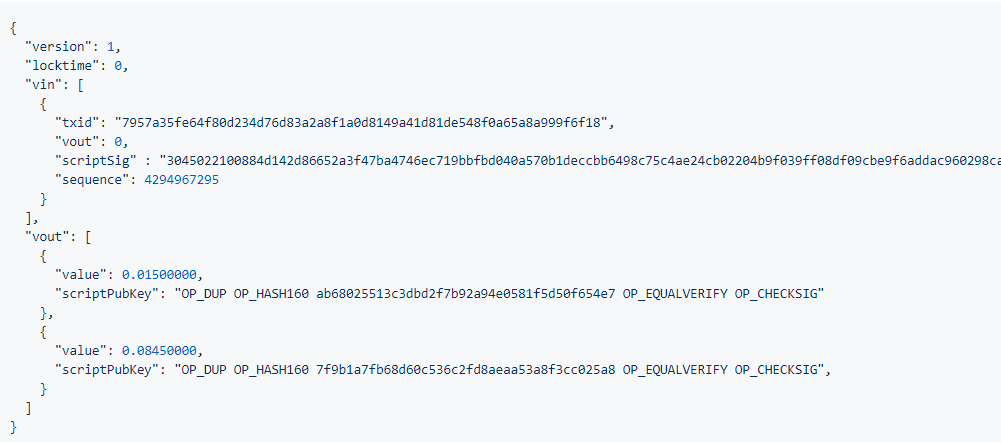
\includegraphics[width=\textwidth]{btc-tx.png}
    \end{center}
    \caption{A decoded Bitcoin transaction} \label{fig:btc-tx}
\end{figure}

A transaction is valid if the following conditions are fulfilled:

\begin{itemize}
    \item The total value of inputs is greater than or equal to the total value of outputs.
    \item For all $\varUTXO \opIn \varBtcInputs$ $\procVerfUTXO{\varUTXO} \opEqNoQ 1$ must hold.
    \item All input UTXOs have not been spent before.
    \item If a locktime $\varTime$ is given, the Bitcoin blockchain's current block needs to be higher or equal $\varTime$.
\end{itemize}

\begin{definition}[Bitcoin Transaction Scheme]
    We define a Bitcoin Transaction Scheme as a tuple of two DPT functions $(\procBuildTransactionId, \procVerfTransactionId)$ and the PPT function $\procSignTransactionId$.
    \begin{itemize}
        \item $\varBtcTx \opFunResult \procBuildTransaction{\varBtcInputs}{\varBtcOutpus}{\varVersion}{\varTime}$: The transaction building algorithm is a DPT function that takes as input a set of unspent transaction outputs $\varBtcInputs$, a collection of newly created transaction outputs $\varBtcOutpus$ a version number $\varVersion$ and an optional locking time $\varTime$.
        The algorithm will output an unsigned transaction $\varBtcTx$.
        \item $\funStar{\varBtcTx} \opFunResult \procSignTransaction{\varBtcTx}{\funArray{\varScriptSig}}$: The transaction
        signing algorithm is a PPT function that takes as input an unsigned Bitcoin transaction $\varBtcTx$ and an array
        of unlocking scripts $\funArray{\varScriptSig}$ for all transaction inputs.
        The algorithm outputs a signed Bitcoin transaction, which the sender can now broadcast to the network.
        \item $\{ 1,0 \} \opFunResult \procVerfTransaction{\varBtcTx}$: The verification algorithm is a DPT function taking as input a transaction $\varBtcTx$ outputting 1 on a successful verification or 0 otherwise.
        The function will check the well-balancedness of the transaction, verify the unlocking scripts, locktime and scan through the blockchain if all inputs are indeed unspent.
        Note that any public verifier with access to the blockchain ledger and $\varBtcTx$ is able to perform the verification.
    \end{itemize}
\end{definition}

We now outline two common structures of Bitcoin outputs the P2PK/P2PKH and the P2SH outputs.

\subsubsection{P2PK, P2PKH\label{sec:pre:bitcoin:p2pk}}

P2PK stands for Pay-to-Public-Key, and P2PKH for Pay-to-Public-Key-Hash.
In \removepms{this}\newpms{the former} type of output $\varScriptPubKey$ will be constructed such that its value unlocks if a correct signature is provided in $\varScriptSig$ for a corresponding public key $\varPubKey$.
P2PKH is an update to this script in which the $\varScriptPubKey$ contains a hashed version of the public key $\varPubKey$ instead of the public key itself.
To spend a P2PKH output, one has to provide the unhashed public key in addition to a valid signature.
This type of output is the most commonly used output in the Bitcoin blockchain to transfer value from one participant to another.
Delgado et al. found in their paper Analysis of the Bitcoin UTXO set~\cite{delgado2018analysis} from 2017 that more than 80\% of the UTXO set consisted of P2PKH transactions, whereas about 17\% were P2SH and 0.12\% P2PK outputs.
P2PKH outputs can be encoded into a Bitcoin address using base58 encoding.
These addresses can be handed out to request a payment from somebody.

\subsubsection{P2SH} \label{sec:pre:bitcoin:p2sh}

If more advanced spending conditions, such as multi-signature, are required, P2SH (Pay-to-script-hash), introduced in 2012, is a way to implement those in a space-efficient and straightforward \removepms{matter}\newpms{manner}.
Here the locking condition $\varScriptPubKey$ does not contain a script but instead the hash of a script.
Upon spending, the spender has to provide the original script and the unlocking requirements for the script itself.
Upon verification, the provided script's hash will be computed and compared with the value given in the locking condition.
If those match, the actual script will be executed.
The advantage of using this approach over just handcrafting a custom locking script is that the locking scripts are relatively short, making the transactions smaller, reducing fees, or shifting them from the sender to the output owner.
Additionally, this type of output can be encoded again into a Bitcoin address similar to a P2PKH output, making it easy to request a payment.

\section{Privacy-enhancing Cryptocurrencies} \label{sec:pre:privacy}
\urldef\urlblockexp\url{https://blockstream.info/}
\urldef\urlzcash\url{https://z.cash/}
\urldef\urlmonero\url{https://www.getmonero.org/}

As seen in~\cref{sec:pre:bitcoin} in Bitcoin funds are stored in UTXOs, which an address can identify.
The value being transferred in a transaction is given in plain text; therefore, by the nature of Bitcoin’s public blockchain, anyone can look up the amount stored in a given address.
So-called block explorers\footnote{\urlblockexp} make such a lookup straightforward.
As demonstrated, for instance, in~\cite{barber2012bitter} or~\cite{reid2013analysis}, it is further possible to link multiple addresses by analyzing transactions, further weakening the system's anonymity and allowing for the extraction of sensitive metadata.
Attempts such as CoinJoin~\cite{maxwell2013coinjoin} or its successor CoinShuffle~\cite{ruffing2014coinshuffle}, CoinShuffle++~\cite{ruffing2017p2p} introduced protocols that can mitigate this likability issue in Bitcoin.

The goal of privacy-enhancing cryptocurrencies is to improve upon Bitcoin's anonymity by the use of cryptographic techniques such as Zero-Knowledge Proofs( see~\cref{sec:pre:privacy:zeroknowlegde}) and homomorphic commitments (see~\cref{def:pre:homo-com}) to achieve Transaction Unlinkability as well as Confidential Transaction Amounts (first mentioned by Adam Back in~\cite{back2013confidentialtx}) in which the transferred values are hidden in homomorphic Commitments.

\begin{definition}[Transaction Unlinkability] \label{def:pre:privacy:tx-unlink}
    Given are the two related transactions $\varTx_a$ which sends a value from $A \rightarrow B$, $\varTx_b$ sending from $B \rightarrow C$ and unrelated $\varTx_c$ sending from $X \rightarrow Y$.
For an attacker $\cnstAdversary$ that is given $\varTx_a$, $\varTx_b$, $\varTx_c$ with the task of finding the linking transactions and without having any additonal knowledge than what can be inferred from the public ledger, the following must hold for Transaction Unlinkability to be fulfilled:
    \[ \varProbability(\cnstAdversary(\varTx_a, \varTx_b, \varTx_c) \opEqNoQ (\varTx_a, \varTx_b)) \opEqNoQ \frac{1}{3} \opAddScalar \funNegl{\cdot}\]
\end{definition}

\begin{definition}[Confidential Transaction Amounts] \label{def:pre:privacy:conf-tx}
    Given two transaction amounts $\varAmount_1, \varAmount_2$, randomness $\varBlindingFactor \opFunResult \cnstIntegersPrimeWithoutZero{*}$ and two encrypted transaction amounts $\varCommitment_1 \opFunResult \procCommit{\varAmount_1}{\varBlindingFactor}$, $\varCommitment_2 \opFunResult \procCommit{\varAmount_2}{\varBlindingFactor}$.
For the adversary $\cnstAdversary$ with the task of finding the correct encrypted transaction amount the following must hold:
    \[ \varB \opFunResult \{0,1\} \;\;\; \varProbability(\cnstAdversary(\varAmount_\varB, (\varCommitment_1, \varCommitment_2)) \opEqNoQ \varCommitment_\varB) \opEqNoQ \frac{1}{2} \opAddScalar \funNegl{\cdot} \]
\end{definition}

Notable examples of such constructions are Zerocash~\cite{sasson2014zerocash}, Monero~\cite{noether2015ring}, and Mimblewimble~\cite{jedusor2016mimblewimble}.
Zerocoin proposed using one-way accumulators~\cite{benaloh1993one}, allowing the minting of of unlinkable Zerocoins from regular Bitcoins.
However, their proposal had some limitations, such as only allowing Zerocoins of a fixed denomination and the inefficient construction.
In Zerocash, the authors improved upon Zerocoin by utilizing Zero-Knowledge Succinct Non-interactive Arguments of Knowledge (zk-SNARKs)~\cite{bitansky2012extractable} instead of an accumulator and managed to address the limitations.
However, the protocol requires an initial trusted setup.
A prominent implementation of the Zerocash protocol is the Zcash cryptocurrency.\footnote{\urlzcash}
Monero utilizes Ring Signatures to achieve Transaction Unlinkability and further uses homomorphic Commitments (see~\cref{def:pre:homo-com}) together with range proofs (see~\cref{sec:pre:rangeproof}) to hide transaction amounts as initially proposed by Adam Back.
The Monero protocol has been implemented in the Monero cryptocurrency.\footnote{\urlmonero}
Mimblewimble, being the main topic of this thesis, will be discussed in detail in~\cref{sec:pre:mimblewimble}.

\subsection{Zero-Knowledge Proofs} \label{sec:pre:privacy:zeroknowlegde}

Zero-Knowledge proofs were first defined in 1988 by Fiat, Fiege, and Shamir and are essential for building cryptocurrencies.
The proofs allow a prover to convince a verifier that he owns a witness value without revealing the value itself.
Initially, the protocol was presented as an interactive proof between a prover and verifier.
However, by utilizing the Fiat Shamir Heuristic~\cite{feige1988zero}, the proofs can be converted into a non-interactive protocol, making the proof publicly verifiable.
Digital signatures (see~\cref{def:pre:signature-scheme}) such as Schnorr Signatures are a prominent instantiation of a Zero-Knowledge proof protocol.
Zero-Knowledge proofs such as Bulletproofs~\cite{bunz2018bulletproofs}, or zk-SNARKS~\cite{bitansky2012extractable}, have essential applications in privacy-enhancing cryptocurrencies.


\subsection{Range Proofs} \label{sec:pre:rangeproof}

A range proof testifies that a secret value that was encrypted or committed to lies within a specific valid range of values.
The proofs are Zero-Knowledge in that they do not leak any information about the secret value other than that it lies in the given interval~\cite{bunz2018bulletproofs}.
Range proofs can be implemented using ring signatures~\cite{noether2016ring}, which was the original implementation used by Monero, later replaced by the more efficient Bulletproofs~\cite{bunz2018bulletproofs}, which are also used in the two most prominent Mimblewimble-based cryptocurrencies, Beam and Grin.
We define a Range Proof System as follows:

\begin{definition}[Range Proof System]\label{def:pre:rangeproof}
    A Range Proof System $\varRProofSystemParam{\varCommitScheme}$ regarding a homomorphic Commitment Scheme $\varCommitScheme$ consists of a tuple of functions $(\procRProofSetupId,$ $\procProofId, \procVerfProofId)$.
    \begin{asparaitem}
        \item $\varRProofParams \opFunResult \procRProofSetup{\varSecParam}{\varI}{\varJ}$: The range proof setup algorithm takes as input a security parameter $\varSecParam$ and two numbers $\varI$ and $\varJ$ to define the lower and upper bound $(\varLowerBound, \varUpperBound)$ of the range proof protocol.
        \item $\varProof \opFunResult \procProof{\varCommitment}{\varValue}{\varBlindingFactor}$: The proof algorithm is a PPT function that takes as input a Commitment $\varCommitment$, a value $\varValue$ and a blinding factor $\varBlindingFactor$.
        It will output a proof $\varProof$ attesting that the value $\varValue$ of Commitment $\varCommitment$ is in between the range $\langle \varLowerBound, \varUpperBound \rangle$ as defined during the $\procRProofSetupId$ function.
        \item $\{1,0\} \opFunResult \procVerfProof{\varProof}{\varCommitment}$: The proof verification algorithm is a DPT function that verifies the validity of the proof $\varProof$ concerning the Commitment $\varCommitment$.
        It will output 1 upon a successful verification or 0 otherwise.
    \end{asparaitem}
\end{definition}

An efficient instantion of a Range Proof System is the bulleproof~\cite{bunz2018bulletproofs} protocol that is currently used in the Monero and Mimblewimble-based cryptocurrencies.

We also define a Two-Party Range Proof System as an extension to a regular Range Proof System.
Two parties collaborate to compute a Zero-Knowledge proof attesting that a secret value of a specific Commitment or encrypted value is within a given interval.
A construction of such a protocol was done, for instance, by Klinec et al. in~\cite{klinec2020privacy}.

\begin{definition}[Two-Party Range Proof System]\label{def:pre:mp-rangeproof}
    A Two-Party Range Proof System $\varMPRProofSystemParam{\varCommitScheme}$ regarding a homomorphic Commitment Scheme $\varCommitScheme$ is an extension to the regular Range Proof System with the following
    distributed protocol $\procDRProofId$.
    \begin{asparaitem}
        \item $\varProof \opFunResult \procDRProof{\varCommitment}{\varValue}{\varBlindingFactorAlice}{\varBlindingFactorBob}$: The distributed proof protocol allows two parties Alice and Bob, each owning a share of the
        Commitment $\varCommitment$, to cooperate to produce a valid range proof $\varProof$ without a party learning the blinding factor share from the other party.
    \end{asparaitem}
\end{definition}

We require both our Range Proof System and the Two-Party Range Proof System to fulfill Soundness (as defined in~\cite{morais2019survey}), Completeness (as defined in~\cite{morais2019survey}) and Zero-Knowledge (as defined in~\cite{fuchsbauer2019aggregate}).


\section{Mimblewimble} \label{sec:pre:mimblewimble}
In this section we will outline the fundamental properties of the protocols employed in Mimblewimble which are relevant for the thesis and particularly the construction of the Atomic Swap protocol constructed in chapter~\ref{ch:atomicswap}.
\subsubsection{Transaction Structure} \label{subsec:pre:mimblwimble-tx}

First we will define the notion of a coin in Mimblewimble which has similarity to an unspent transaction output (UTXO) in Bitcoin.
\begin{definition}[Mimblewimble Coin]\label{def:pre:coin}
    For two adjacent elliptic curve generators $\varG$ and $\varH$ a coin in Mimblewimble is a tuple of the form ($\varCoin$, $\varProof$), where $\varCoin \opAssign \funGen{\varValue} \opAddPoint \funGenH{\varNonce}$ is a Pedersen Commitment~\cite{pedersen1991non}
    to the value $\varValue$ with blinding factor $\varNonce$. $\varProof$ is a range proof attesting to the statement that $\varValue$ is in a valid range in zero-knowledge.
    The valid range is defined by the specific implementation, in pratice $\langle 0, 2^{64} -1 \rangle$ is used in the most prominant implementations.
\end{definition}

A Mimblewimble transaction consists of $\varCoinInp \opAssign (\varCoin_1 , \dots , \varCoin_n)$ input coins, $\varCoinOut \opAssign (\varCoin'_1 , \dots , \varCoin'_n)$ output coins and kernel $\varKernel$, which we will define throughout this section.
\begin{definition}[Transaction well-balancedness]  \label{def:pre:tx-well-balancedness}
    A transaction is considered \emph{well-balanced} if $\sum{\varValue'_i} \opSub \sum{\varValue_i} \opEqNoQ 0$ so the sum of all output values subtracted from the sum of input values has to be 0. (Not taking transaction fees into account)
\end{definition}

\begin{definition}[Transaction validity] \label{def:pre:tx-mw-validity}
    A transaction is valid if:
    \begin{itemize}
        \item The transaction is well-balanced as defined in definition~\ref{def:pre:tx-well-balancedness}
        \item $\opForAll \; (\varCoin_i \varProof_i) \opIn \varCoinOut \; \procVerfProof{\varProof_i}{\varCoin_i} \opEqNoQ 1$
    \end{itemize}
\end{definition}

From the definition of \emph{Transaction validity} we can derive the following equation:
\[ \sum{\varCoinOut} \opSub \sum{\varCoinInp} \opEqNoQ \sum{(\funGenH{\varValue'_i} \opAddPoint \funGen{\varNonce'_i})} \opSub \sum{(\funGenH{\varValue_i} \opAddPoint \funGen{\varNonce_i})} \]
So if we assume that a transaction is valid then we are left with the following so called excess value:
\[ \varExcess \opEqNoQ \funGen{\varExcessExp} \opEqNoQ \funGen{(\sum{\varNonce'_i} \opSub \sum{\varNonce_i})} \]
Knowledge of the opening of all coins, and the well-balancedness of the transaction implies knowledge of the discrete logarithm $\varExcessExp$ of $\varExcess$.
Directly revealing $\varExcessExp$ would leak too much information, an adversary knowing the openings for input coins and all but one output coin, could easily calculate the unknown opening given $\varExcessExp$.
Therefore instead knowledge of the discrete logarithm to $\varExcess$ is proven by providing a valid signature for $\varExcess$ as public key.
Finally we would like to add that coinbase transactions (transactions creating new money as part of mining reward) additionally include the newly minted money as supply $\varSupply$ in the excess equation as follows:
\[ \varExcess \opAssign \funGen{(\sum{\varNonce'_i} \opSub \sum{\varNonce_i})} \opSub \funGenH{\varSupply} \]
For non coinbase transactions, $\varSupply$ will simply be set to 0.
Finally, a Mimblewimble transaction is of form:
\[ \varTx \opAssign (\varSupply \opSeperate \varCoinInp \opSeperate \varCoinOut \opSeperate \varKernel)\:\text{with}\:\varKernel \opAssign (\funList{\varProof} \opSeperate \funList{\varExcess} \opSeperate \funList{\varSignature}) \]
where $\varSupply$ is the transaction supply amount, $\varCoinInp$ is the list of input coins, $\varCoinOut$ is the list of output coins and $\varKernel$ is the transaction Kernel.
The Kernel consists of $\funList{\varProof}$ which is a set of all output coin range proofs, $\funList{\varExcess}$ a set of excess values and finally $\funList{\varSignature}$ a set of signatures ~\cite{fuchsbauer2019aggregate}.
Even though normally a transaction would only require a single excess value and signature, for reasons we will see in the next section these fields always have to be lists instead of just a single value.

\subsubsection{Transaction Merging \label{sec:pre:mimblewimble:merge}}
An intriging property of the Mimblewimble protocol is that two transactions can easily be merged into a single one, which is essentially a non-interactive version of the CoinJoin protocol on Bitcoin~\cite{maxwell2013coinjoin}.
Assume we have the following two transactions:
\begin{gather*}
    \varTx_0 \opAssign (\varSupply_0 \opSeperate \varCoinInp^0 \opSeperate \varCoinOut^0 \opSeperate (\funList{\varProof_0} \opSeperate \funList{\varExcess_0} \opSeperate \funList{\varSignature_0}) )\\
    \varTx_1 \opAssign (\varSupply_1 \opSeperate \varCoinInp^1 \opSeperate \varCoinOut^1 \opSeperate (\funList{\varProof_1} \opSeperate \funList{\varExcess_1} \opSeperate \funList{\varSignature_1}) )\\
\end{gather*}
Then we can build a single merged transaction:
\[ \varTx_m \opAssign (\varSupply_0 \opAddScalar \varSupply_1 \opSeperate \varCoinInp^0 \opConc \varCoinInp^1,\:\varCoinOut^0 \opConc \varCoinOut^1 \opSeperate (\funList{\varProof_0} \opConc \funList{\varProof_1} \opSeperate
\funList{\varExcess_0} \opConc \funList{\varExcess_1} \opSeperate \funList{\varSignature_0} \opConc \funList{\varSignature_1}) \]
We can easily deduce that if $\varTx_0$ and $\varTx_1$ are valid, it must follow that $\varTx_m$ is valid:\\
If $\varTx_0$ and $\varTx_1$ are valid as of definition~\ref{def:pre:tx-mw-validity} that means $\varCoinInp^0 \opSub \varCoinOut^0 \opSub \funGenH{\varSupply_0} \opEqNoQ \varExcess_0 \opSeperate \funList{\varProof_0}$ contains valid range proofs for the outputs
$\varCoinOut^0$ and $\funList{\varSignature_0}$ contains a valid signature to $\varExcess_0 \opSub \funGenH{\varSupply_0}$ as public key, the same must hold for $\varTx_1$.

By the rules of arithmetic it then must also hold that
\[ \varCoinInp^0 \opConc \varCoinInp^1 \opSub \varCoinOut^0 \opConc \varCoinOut^1 \opSub \funGenH{\varSupply_0 \opAddScalar \varSupply_1} \opEqNoQ \varExcess_0 \opAddPoint \varExcess_1  \]
$\funList{\varProof_0} \opConc \funList{\varProof_1}$ must contain valid range proofs for the output coins and $\funList{\varSignature_0} \opConc \funList{\varSignature_1}$ must contain valid signatures to the respective Excess points, which makes $\varTx_m$ a valid transaction.

\paragraph{Subset Problem} \label{par:pre:mimblewimble:subset}
A subtle problem arises with the way transactions are merged in Mimblewimble.
From the construction shown earlier, it is possible to reconstruct the original separate transactions from a merged one, which can be a privacy issue.
Given a set of inputs, outputs, and kernels, a subset of these will recombine to reconstruct one of the valid transaction which were aggregated since kernel excess values are not combined.
Recall the merged transaction from earlier:
\[ \varTx_m \opAssign (\varSupply_0 \opAddScalar \varSupply_1 \opSeperate \varCoinInp^0 \opConc \varCoinInp^1,\:\varCoinOut^0 \opConc \varCoinOut^1 \opSeperate (\funList{\varProof_0} \opConc \funList{\varProof_1}) \opSeperate
\funList{\varExcess_0} \opConc \funList{\varExcess_1} \opSeperate \funList{\varSignature_0} \opConc \funList{\varSignature_1}) \]
Since the attacker has access to both $\varExcess_0$ and $\varExcess_1$ as well as $\varSignature_0$ and $\varSignature_1$, he can simply try different combinations of input values $\funStar{\funList{\varCoinInp}}$ and output values $\funStar{\funList{\varCoinOut}}$ until he finds a combination under which the transaction is valid with $\varExcess_0, \varSignature_0$ or $\varExcess_1, \varSignature_1$.
Thereby the attacker was able to reconstruct one of the original transactions from which $\varTx_m$ was constructed.
Following this method he might be able to uncover all original transactions from the merged one.

This problem has been mitigated in cryptocurrencies implementing the protocol by including an additional variable $\varOffset$ in the Kernel, called offset value.
Briefly recall the construction of the excess value $\varExcess$:
\[ \varExcess \opAssign \funGen{\varExcessExp} \]
In order to solve the problem we redefine $\varExcess$ as:
\[ \varExcess \opAssign \funGen{\varExcessExp \opSub \varOffset} \]
Since $\varOffset$ is now also included in the transaction kernel and therefore known to the verifier, the public verification is still possible.
Now every time two transactions are merged with the method layed out previously, the two individual offset values $\varOffset_0, \varOffset_1$ are combined into a single value $\varOffset_m$.
If offsets are picked truly randomly, and the possible range of values is broad enough, the probability of recovering the uncombined offsets from a merged one becomes negligible, making it infeasible to recover original transactions from a merged one~\cite{poelstra2016mimblewimble}.


\paragraph{Cut Through} \label{par:pre:mimblewimble:cut}
From the way transactions are merged together, we can now learn how to purge spent outputs securely.
Let's assume $\varCoin_i$ appears as an output in $\varTx_0$ and as an input in $\varTx_1$:
\begin{gather*}
    \varTx_0 \opAssign (\varSupply_0 \opSeperate \varCoinInp^0 \opSeperate \varCoinOut^i \opSeperate (\funList{\varProof_0} \opSeperate \funList{\varExcess_0} \opSeperate \funList{\varSignature_0}) )\\
    \varTx_1 \opAssign (\varSupply_1 \opSeperate \varCoinInp^i \opSeperate \varCoinOut^1 \opSeperate (\funList{\varProof_1} \opSeperate \funList{\varExcess_1} \opSeperate \funList{\varSignature_1}) )\\
\end{gather*}
Essentially this means $\varTx_1$ spends a coin created in $\varTx_0$.
Now lets recall the equation given for transaction well-balancedness in~\ref{def:pre:tx-well-balancedness}:
\[ \sum{\varCoinOut} \opSub \sum{\varCoinInp} \opEqNoQ \sum{(\funGen{\varNonce'_i})} \opSub \sum{(\funGen{\varNonce_i})} \]
If we merge $\varTx_0$ with $\varTx_1$ as done previously the coin $\varCoin_i$ will appear both in $\sum{\varCoinInp}$ and $\sum{\varCoinOut}$.
Therefore we can erase $\varCoin_i$ from both lists, while maintaining transaction balancedness.
Informally this means that every time a coin gets spend, it can be erased from the ledger, without breaking the rules of the system.
This property is employed in the Mimblewimble protocol to reduce the space requirements of the protocol as well as provide a notion of unlinkability, as transaction histories can be erased.

\subsubsection{Transaction Building} \label{subsec:pre:mimblewimble:txbuild}
As already pointed out, building transactions in Mimblewimble is an interactive process between the sender and receiver of funds.
Jedusor, Tom Elvis originally envisioned the following two-step process to build a transaction:~\cite{jedusor2016mimblewimble}

Throughout the thesis whenever we are concerned with Mimblewimble transactions we generally refer to the sending party (owning the input coins) as Alice and the receiving party (owning the newly created output coin) as Bob.
Assume for the following that Alice wants to transfer coins of value $\varFundValue$ to Bob:
\begin{enumerate}
    \item Alice first selects an input coin $\varCoinInp$ (or potentially multiple) in her control with total stored value $\varValue$ with $\varValue \geq \varFundValue$.
    She then creates change coin outputs $\varCoinOutAlice$ (could again be multiple) with the remainder of her input value substracted by the value send to Bob.
    For her newly created output coins and her input coins she calculates her part of discrete logarithm $\varKey$ (her part of the key) to the final $\varExcess$ and sends all this information to Bob as a pre-transaction.
    \item Bob creates himself additional output coins $\varCoinOut^B$ of total value $\varFundValue$ and similar to Alice creates his share $\funStar{\varKey}$ of the discrete logarithm of $\varExcess$.
    Together with the share received by Alice he can now create a signature to $\varExcess$ and finalize the transaction
\end{enumerate}
Figure~\ref{fig:txOriginal} depicts the original transaction flow.\\
\begin{figure}
    \centering
    \pseudocode[codesize=\scriptsize]{
        \textbf{Alice} \< \< \< \< \textbf{Bob} \\ [][\hline]
        \< \< \< \< \\
        \text{ Select $\varCoinInp$ of value $\varValue \geq \varFundValue$ } \< \< \< \< \\
        \text{ Create $\varCoinOutAlice$ of value $\varValue \opSub \varFundValue$} \< \< \< \< \\
        \text{ $\varExcess_{A} \opAssign \sum{\varCoinOutAlice} \opSub \sum{\varCoinInp}$ } \\
        \text{ $(-\varFundValue \opSeperate \varKey)$ opening to $\varExcess_{A}$ } \< \< \< \< \\
        \text{ Create range-proof $\varProof$ for $\varCoinOutAlice$ } \< \< \< \< \\
        \< \sendmessageright{ top=$(-\varFundValue \opSeperate \varKey) \opSeperate \varProof$ } \< \< \< \\
        \< \< \< \< \text{Create $\varCoinOut^B$ with value $\varFundValue$ and keys $(\varKeySt_i)$ } \\
        \< \< \< \< \text{$\varKey_{shared} \opAssign \varKey \opAddScalar \sum{\varKeySt_i}$ } \\
        \< \< \< \< \text{Create $\varSignature$ with $\varKey_{shared}$} \\
        \< \< \< \< \text{ Create range-proof $\varProof$ for $\varCoinOutBob$ } \\
        \< \< \< \< \text{Finalize transaction $\varTx$} \\
    }
    \caption{Original transaction building process\label{fig:txOriginal}}
\end{figure}

This protocol however turned out to be insecure as it is vulnerable to the following attack:
The receiver could spend Alice's change coins $\varCoinOut^A$ by reverting the transaction.
Doing this would give the sender his coins back, however as the sender might not have the keys for his spent outputs anymore, the coins could then be lost.

In detail this reverting transaction would look like:
\[ \varTx_{rv} \opAssign (0 \opSeperate \varCoinOut^A \opConc \varCoinOut^B \opSeperate \varCoinInp \opSeperate (\varProof_{rv} \opSeperate \varExcess_{rv} \opSeperate \varSignature_{rv}) ) \]
So in essence it is exactly the reverse of the previous transaction.
Again remembering the construction of the excess value of this construction would look like this:
\[ \varExcess_{rv} \opAssign \sum{\varCoinOut^A \opConc \varCoinOut^B \opSub \varCoinInp} \]
The key $\varKey$ originally sent by Alice to Bob is a valid opening to $\sum{\varCoinInp} \opSub \sum{\varCoinOut^A}$. With the inverse of this key $\varKey_{inv}$ we get the opening to $\sum{\varCoinOut^A \opSub \varCoinInp}$.
Now all Bob has to do is add his key $\funStar{\varKey}$ to get:
\[ \varKey_{rv} \opAssign -\varKey \opAddScalar \funStar{\varKey} \]
which is the opening to $\varExcess_{rv}$.
Therefore Bob is able to construct a valid signature under $\varExcess_{rv}$.
Range proofs can just be reused, because this transaction spends to a coin which has already existed on the ledger with the same blinding factor and value, meaning the proof will still be valid.

In essence this means Bob spends the newly created outputs and sends them back to the original input coins, chosen by Alice. It might at first seem unclear why Bob would do that.
An example situation could be if Alice pays Bob for some good which Bob is selling. Alice decides to pay in advance, but then Bob discovers that he is already out of stock of the good that Alice ordered.
To return the funds to Alice, he reverses the transaction instead of participating in another interactive process to build a new transaction with new outputs.
If Alice already deleted the keys to her initial coins, the funds are now lost.
The problem was solved in the Grin and Beam Mimblewimble implementations by making the signing process itself a two-party process which will be explained in more detail in chapter~\ref{ch:fixedwitnesssignatures}.

Alternatively Fuchsbauer et al.~\cite{fuchsbauer2019aggregate} proposed another way to build transactions which would not be vulnerable to this problem:
\begin{enumerate}
    \item Alice constructs a full-fledged transaction $\varTx_A$ spending her input coins $\varCoinInp$ and creates her change coins $\varCoinOut^A$, plus a special output coin $\varCoinSpecial \opAssign \funGenH{\varFundValue} \opAddPoint \funGen{\varKey_{sp}}$,
    where $\varFundValue$ is the desired value which should be transferred to Bob and $\varKey_{sp}$ is a randomly choosen key. She proceeds by sending $\varTx_A$ as well as $(\varFundValue \opSeperate \varKey_{sp})$ and the necessary range
    proofs to Bob.
    \item Bob now creates a second transaction $\varTx_B$ spending the special coin $\varCoinSpecial$ to create an output only he controls $\varCoinOutBob$ and merges $\varTx_A$ with $\varTx_B$
    into $\varTx_m$. He then broadcasts $\varTx_m$ to the network. Note that when the two transactions are merged the intermediate special coin $\varCoinSpecial$ will be both in the coin output and input list
    of the transaction and therfore will be discarded.
\end{enumerate}
One drawback of this approach is that we have two transaction kernels instead of just one because of the merging step, making the transaction slightly bigger, however there is still only one interaction required between Alice and Bob.
In the solution employed by the Grin and Beam implementations which we will discuss in chapter~\ref{ch:atomicswap}, at least one additional round of interaction will be required.
A figure showing the protocol flow is depicted in Figure~\ref{fig:txSalvaged}.

\begin{figure}
    \centering
    \pseudocode[codesize=\scriptsize]{
        \textbf{Alice} \< \< \< \< \textbf{Bob} \\ [][\hline]
        \< \< \< \< \\
        \text{ Select $\varCoinInp$ of value $\varValue \geq \varFundValue$ } \< \< \< \< \\
        \text{ Create $\varCoinOutAlice$ of value $\varValue \opSub \varFundValue$ } \< \< \< \< \\
        \varKey_{sp} \sample \cnstIntegersPrimeWithoutZero{\varPrime} \< \< \< \< \\
        \text{ Create $\varCoinSpecial \opAssign \funGenH{\varFundValue} \opAddScalar \funGen{\varKey_{sp}}$ } \< \< \< \< \\
        \text{ Construct and sign $\varTxAlice$ with $\varCoinInp \opSeperate \varCoinOutAlice \opSeperate \varCoinSpecial$ } \< \< \< \< \\
        \< \sendmessageright{ top=$\varTxAlice \opSeperate \varFundValue \opSeperate \varKey_{sp}$ } \< \< \< \\
        \< \< \< \< \text{ Create $\varCoinOut^B$ with value $\varFundValue$ } \\
        \< \< \< \< \text{ Create $\varTxBob$ spending $\varCoinSpecial$ to $\varCoinOut^B$ } \\
        \< \< \< \< \text{ Merge $\varTxAlice$ and $\varTxBob$ to $\varTx_{m}$ } \\
        \< \< \< \< \text{ Publish $\varTx_{m}$ }
    }
    \caption{Salvaged transaction protocol by Fuchsbauer et al.~\cite{fuchsbauer2019aggregate} \label{fig:txSalvaged}}
\end{figure}



\section{Scriptless Scripts} \label{sec:pre:scriptless-scripts}
In 2017 Andrew Poelstra presented a concept called Scriptless Scripts that achieves the execution of primitive contracts only by the use of standard cryptographic tools such as digital signatures.~\cite{poelstra2017scriptless}
The most prominent Scriptless Script is the Adaptor Signature Scheme which has been fully formalized and proven to be secure for Schnorr and ECDSA by Aumayr et al. in~\cite{aumayr2020bitcoinchannels}.
Scriptless Scripts are useful for Cryptocurrencies that lack scripting functionality, and such is the case for instance in Mimblewimble based systems, but also helps to replace script-based approaches with improvements in privacy as well as efficiency, shown in a paper by Christoph Egger et al. ~\cite{egger2019atomic}.
In~\cref{ch:fixedwitnesssignatures}, we will leverage the Adaptor Signature Scheme concept together with a Two-Party Signature Scheme to build a scriptless Atomic Swap protocol applicable for Mimblewimble based Cryptocurrencies.
The Adaptor Signature Scheme is a two-step process.
A signer first computes a pre-signature that can be completed only by a party knowing a certain secret witness value $\varWit$ from a hard relation $(\varWit, \varStatement) \opIn \cnstRelation$.
After the pre-signature is completed into the final one, it must then be possible to extract $\varWit$ given the final and the pre-signature.

We here repeat the definition of an Adaptor Signature Scheme found by Aumayr et al. in~\cite{aumayr2020bitcoinchannels}.

\begin{definition}[Adaptor Signature Scheme]\label{def:pre:script:apt}
    An Adaptor Signature Scheme wrt. a hard relation $\cnstRelation$ and a Signature Scheme $\varSigScheme$ as of~\cref{def:pre:signature-scheme} consists of four algorithms:
    \begin{itemize}
        \item $\funTilde{\varSignature} \opFunResult \styleFunction{pSign}(\varSecKey, \varMsg, \varStatement)$ is a PPT algorithm that on input secret key $\varSecKey$, message $\varMsg \opIn \cnstBinary{*}$ and statement $\varStatement$ outputs a pre-signature $\funTilde{\varSignature}$.
        \item $\cnstTrueorFalse \opFunResult \styleFunction{pVrfy}(\varPubKey, \varMsg, \varStatement, \funTilde{\varSignature})$ is DPT algorithm that on input a public key, message $\varMsg \opIn \cnstBinary{*}$, statement $\varStatement$ and pre-signature $\funTilde{\varSignature}$, outputs either 1 or 0.
        \item $\varSignature \opFunResult \styleFunction{Adapt}(\funTilde{\varSignature}, \varWit)$ is a DPT algorithm that on input a pre-signature $\funTilde{\varSignature}$ and witness value $\varWit$, outputs a signature $\varSignature$.
        \item $\varWit \opFunResult \styleFunction{Ext}(\varSignature, \funTilde{\varSignature}, \varStatement)$ is a DPT algorithm that on input a signature $\varSignature$, pre-signature $\funTilde{\varSignature}$ and statement $\varStatement$, outputs a witness $\varWit$ such that $(\varWit, \varStatement) \opIn \cnstRelation$, or $\cnstFalsum$.
    \end{itemize}
\end{definition}


